\documentclass[tikz,border=2pt]{standalone}
\renewcommand{\familydefault}{\sfdefault}
\usetikzlibrary{arrows.meta,calc,positioning}
\tikzset{every picture/.style={line width=1pt, >=Stealth},
         hl/.style={fill=black, fill opacity=0.12, text opacity=1}}
\begin{document}
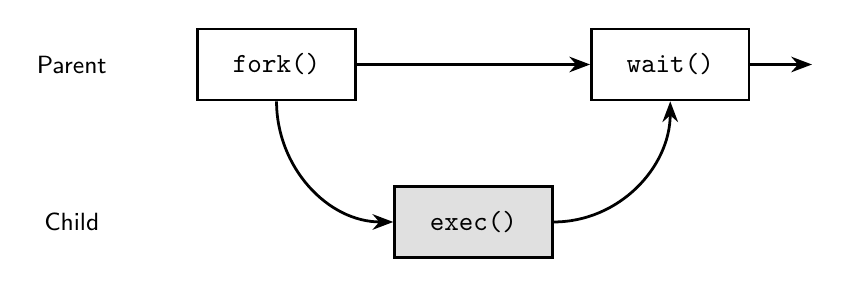
\begin{tikzpicture}[call/.style={draw, minimum width=2cm, minimum height=0.9cm, font=\ttfamily}]
  \node[font=\small] at (0, 0) {Parent};
  \node[font=\small] at (0, -2) {Child};
  \node[call] (fork) at (2.6, 0) {fork()};
  \node[call] (wait) at (7.6, 0) {wait()};
  \node[call, hl] (exec) at (5.1, -2) {exec()};
  \draw[->] (fork) -- (wait);
  \draw[->] (wait) -- ++(1.8, 0);
  \draw[->] (fork.south) to[out=-90, in=180] (exec.west);
  \draw[->] (exec.east) to[out=0, in=-90] (wait.south);
\end{tikzpicture}
\end{document}
